\subsection{Deep Learning}

Deep learning techniques, such as convolutional neural networks (CNNs), can be applied to spectral data for feature extraction and classification. These methods can learn complex relationships in the data and provide robust predictions of carbon levels based on spectral readings. The most important difference between deep learning and the previous methods is that it requires a large amount of training data to be effective. One method by Kim et al. \cite{kim_deep_2025} uses a deep learning model to predict existence, concentration and carbon peak areas.

\begin{figure}[H]
\centering
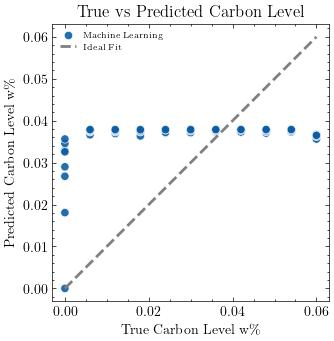
\includegraphics[width=0.8\textwidth]{../Figures/Analysis/carbon_level_vs_predicted_ml_optimization.jpg}
\caption{Deep learning prediction results showing carbon level vs predicted values using machine learning optimization}
\label{fig:ml_predictions}
\end{figure}